\begin{tikzpicture}[
    >=Latex,
    node distance=1.6cm and 0.7cm,
    every node/.style={font=\small},
    stage/.style={
        rectangle, rounded corners=3pt, draw, thick,
        fill=blue!8, minimum width=2.4cm, minimum height=1.7cm,
        align=center, inner sep=4pt,
    },
    flow/.style={->, very thick, blue!50!black},
    flowlabel/.style={font=\scriptsize, gray!70!black, fill=white,
                      inner sep=2pt, align=center},
    iolabel/.style={font=\scriptsize\bfseries, gray!70!black,
                    align=center},
]
    % =========================================================
    % Reihe 1: Stufen 1 bis 4
    % =========================================================
    \node[stage] (s1) {%
        \textbf{1}\\[-2pt]
        \scriptsize Planare Basisschichten\\[2pt]
        \begin{tikzpicture}[baseline]
            \fill[gray!20] (0, 0) rectangle (0.6, 0.4);
            \draw (0, 0) rectangle (0.6, 0.4);
            \foreach \y in {0.1, 0.2, 0.3} {
                \draw[blue!70!black, thin] (0, \y) -- (0.6, \y);
            }
        \end{tikzpicture}
    };

    \node[stage, right=of s1] (s2) {%
        \textbf{2}\\[-2pt]
        \scriptsize Mesh-Verfeinerung\\[2pt]
        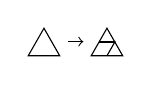
\begin{tikzpicture}[baseline]
            \draw (0, 0) -- (0.4, 0) -- (0.2, 0.35) -- cycle;
            \draw[->, thin] (0.5, 0.18) -- (0.7, 0.18);
            \draw (0.8, 0) -- (1.2, 0) -- (1.0, 0.35) -- cycle;
            \draw (0.9, 0.175) -- (1.1, 0.175) -- (1.0, 0);
            \draw (0.9, 0.175) -- (1.1, 0.175);
        \end{tikzpicture}
    };

    \node[stage, right=of s2] (s3) {%
        \textbf{3}\\[-2pt]
        \scriptsize $\Phi$ lösen\\[2pt]
        \begin{tikzpicture}[baseline]
            \shade[bottom color=viridisLow, top color=viridisHigh,
                   middle color=viridisMid]
                (0, 0) rectangle (0.6, 0.4);
            \draw (0, 0) rectangle (0.6, 0.4);
        \end{tikzpicture}
    };

    \node[stage, right=of s3] (s4) {%
        \textbf{4}\\[-2pt]
        \scriptsize Iso-Extraktion\\[2pt]
        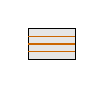
\begin{tikzpicture}[baseline]
            \fill[gray!20] (0, 0) rectangle (0.6, 0.4);
            \draw (0, 0) rectangle (0.6, 0.4);
            \draw[orange!80!black, thin] (0, 0.1) -- (0.6, 0.1);
            \draw[orange!80!black, thin] (0, 0.2) -- (0.6, 0.2);
            \draw[orange!80!black, thin] (0, 0.3) -- (0.6, 0.3);
        \end{tikzpicture}
    };

    % =========================================================
    % Reihe 2: Stufen 5 bis 8
    % =========================================================
    \node[stage, below=1.6cm of s1] (s5) {%
        \textbf{5}\\[-2pt]
        \scriptsize Branch-Tracking\\[2pt]
        
\begin{tikzpicture}[baseline]
            \draw[blue!70!black, thick] (0.3, 0) -- (0.3, 0.2);
            \draw[orange!85!black, thick] (0.3, 0.2) -- (0.1, 0.4);
            \draw[green!50!black, thick] (0.3, 0.2) -- (0.5, 0.4);
        \end{tikzpicture}
    };

    \node[stage, right=of s5] (s6) {%
        \textbf{6}\\[-2pt]
        \scriptsize Infill-Generierung\\[2pt]
        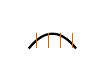
\begin{tikzpicture}[baseline]
            \draw[thick] (0, 0.05) .. controls (0.2, 0.3) and (0.4, 0.3) .. (0.6, 0.05);
            \foreach \x in {0.1, 0.25, 0.4, 0.55} {
                \draw[orange!80!black, very thin]
                    (\x, 0.05) -- (\x, 0.25);
            }
        \end{tikzpicture}
    };

    \node[stage, right=of s6] (s7) {%
        \textbf{7}\\[-2pt]
        \scriptsize Branch-Scheduling\\[2pt]
        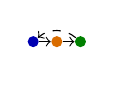
\begin{tikzpicture}[baseline]
            \node[circle, fill=blue!70!black, inner sep=0pt, minimum size=4pt] (a) at (0, 0.2) {};
            \node[circle, fill=orange!85!black, inner sep=0pt, minimum size=4pt] (b) at (0.3, 0.2) {};
            \node[circle, fill=green!50!black, inner sep=0pt, minimum size=4pt] (c) at (0.6, 0.2) {};
            \draw[->, thin] (a) -- (b);
            \draw[->, thin] (b) -- (c);
            \draw[->, thin, dashed] (c) to[bend right=40] (a);
        \end{tikzpicture}
    };

    \node[stage, right=of s7] (s8) {%
        \textbf{8}\\[-2pt]
        \scriptsize \gls{toolpath}-Konstruktion\\[2pt]
        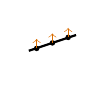
\begin{tikzpicture}[baseline]
            \draw[thick] (0, 0.1) -- (0.6, 0.3);
            \foreach \x/\y in {0.1/0.13, 0.3/0.20, 0.5/0.27} {
                \fill[black] (\x, \y) circle (1pt);
                \draw[->, very thin, orange!85!black]
                    (\x, \y) -- ++(0, 0.12);
            }
        \end{tikzpicture}
    };

    % =========================================================
    % Pfeile (ohne Labels darauf)
    % =========================================================
    \draw[flow] (s1) -- (s2);
    \draw[flow] (s2) -- (s3);
    \draw[flow] (s3) -- (s4);

    \draw[flow] (s5) -- (s6);
    \draw[flow] (s6) -- (s7);
    \draw[flow] (s7) -- (s8);

    % =========================================================
    % Umbruch-Pfeil von s4 zu s5 (explizite Koordinaten)
    % =========================================================
    \coordinate (w1) at ([xshift=0.4cm]s4.east);
    \coordinate (w2) at ([yshift=-1.05cm]w1);
    \coordinate (w3) at (w2 -| s5);
    \draw[flow] (s4.east) -- (w1) -- (w2) -- (w3) -- (s5.north);

    % =========================================================
    % Labels OBERHALB der Boxen (Reihe 1) und der Boxen (Reihe 2)
    % =========================================================
    % Reihe 1
    \node[flowlabel, anchor=south]
        at ([yshift=2pt]$(s1.north east)!0.5!(s2.north west)$)
        {\gls{mesh}};
    \node[flowlabel, anchor=south]
        at ([yshift=2pt]$(s2.north east)!0.5!(s3.north west)$)
        {verfeinertes \gls{mesh}};
    \node[flowlabel, anchor=south]
        at ([yshift=2pt]$(s3.north east)!0.5!(s4.north west)$)
        {$\Phi$, $\nabla\Phi$};

    % Wrap-Label im Zwischenraum
    \node[flowlabel]
        at ($(w2)!0.5!(w3)$)
        {Iso-Schichten};

    % Reihe 2
    \node[flowlabel, anchor=south]
        at ([yshift=2pt]$(s5.north east)!0.5!(s6.north west)$)
        {+ Branch-IDs};
    \node[flowlabel, anchor=south]
        at ([yshift=2pt]$(s6.north east)!0.5!(s7.north west)$)
        {+ \gls{infill}};
    \node[flowlabel, anchor=south]
        at ([yshift=2pt]$(s7.north east)!0.5!(s8.north west)$)
        {Druckreihenfolge};

    % =========================================================
    % Eingabe und Ausgabe
    % =========================================================
    \draw[flow] ([xshift=-0.7cm]s1.west) -- (s1.west);
    \node[iolabel, anchor=east] at ([xshift=-0.75cm]s1.west)
        {\gls{mesh}};

    \draw[flow] (s8.east) -- ([xshift=0.7cm]s8.east);
    \node[iolabel, anchor=west] at ([xshift=0.75cm]s8.east)
        {\gls{toolpath}};

\end{tikzpicture}